\documentclass[a4paper]{scrartcl}
\usepackage[utf8]{inputenc}

\usepackage{scrpage2}
\usepackage{rotating}
\usepackage{listings}
\usepackage{amsmath}
\usepackage{amsfonts}
\usepackage{enumerate}
%\usepackage{mathtools}
\usepackage{hyperref}

\setlength{\parindent}{0mm}

\pagestyle{scrheadings}
\renewcommand{\thesubsection}{\alph{subsection}}
\clearscrheadfoot

\ohead[]{Nikolas Zeitler, Joshua Hartmann, Alexander Diegel}
\cfoot[\pagemark]{\pagemark}

\author{Nikolas Zeitler, Joshua Hartmann, Alexander Diegel}
\title{Maschinelles Lernen Blatt 5}

%INFO bitte mit TODO-tags arbeiten, dann sieht man es im Studio auf der linken seite
%TODO Beispiel 

\begin{document}
\maketitle
\section{Fragen zur Vorlesung}

\begin{enumerate}[a)]
	\item Warum wendet man die Principal Component Analysis (PCA) an? (Zwei Gründe sollten genannt werden.)
	
	\item Was ist der Unterschied zwischen der PCA und der (Fisher) Linear Discriminant Analysis (LDA)?
	
	\item Welcher Abstand soll von der LDA maximiert werden?
	
	\item Warum genügt es nicht, den eben genannten Abstand zu maximieren?
	
	\item Was beschreibt die within-class scatter matrix (Foliensatz 5, Folie 17)?
	
	\item Was beschreibt die between-class scatter matrix (Foliensatz 5, Folie 18)?
	
	\item Man gebe sowohl für PCA als auch LDA an, ob es sich um ein supervised oder unsupervised Lernverfahren
	handelt.
	
	\textbf{PCA}: \\
	\textbf{LCA}:
	
\end{enumerate}

\newpage

\section{Principal Component Analysis – 1}

\begin{enumerate}[(a)]
	\item \hfill
	
	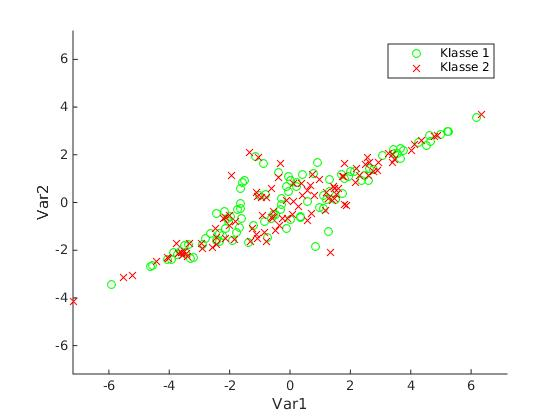
\includegraphics[width=0.75\textwidth]{data/img1.jpg}
		
	\begin{enumerate}
		\item Bietet sich im Allgemeinen eine Dimensionsreduktion auf den PC-Vektor an?
		
		\item Ist dies für die Klassifikation förderlich?
		
	\end{enumerate}
	
	\item \hfill
	
	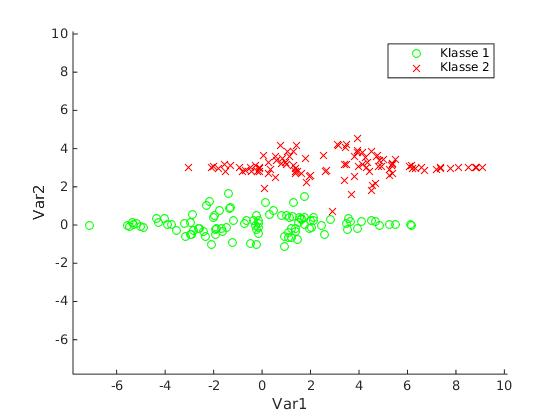
\includegraphics[width=0.75\textwidth]{data/img2.jpg}
	
	\begin{enumerate}
		\item Bietet sich im Allgemeinen eine Dimensionsreduktion auf den PC-Vektor an?
		
		\item Ist dies für die Klassifikation förderlich?
		
	\end{enumerate}
	
	\item \hfill
	
	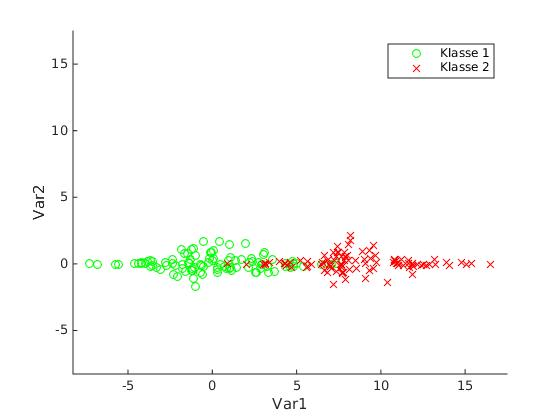
\includegraphics[width=0.75\textwidth]{data/img3.jpg}
	
	\begin{enumerate}
		\item Bietet sich im Allgemeinen eine Dimensionsreduktion auf den PC-Vektor an?
		
		\item Ist dies für die Klassifikation förderlich?
		
	\end{enumerate}
	
	\item \hfill
	
	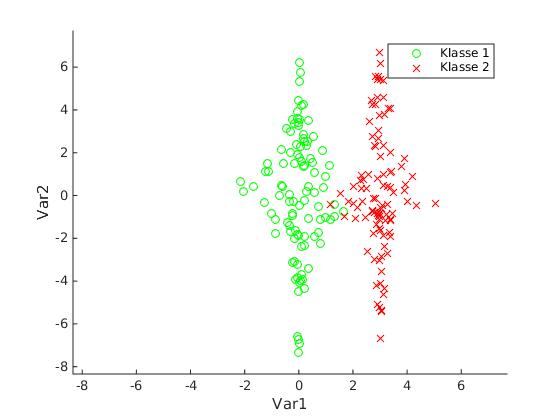
\includegraphics[width=0.75\textwidth]{data/img4.jpg}
	
	\begin{enumerate}
		\item Bietet sich im Allgemeinen eine Dimensionsreduktion auf den PC-Vektor an?
		
		\item Ist dies für die Klassifikation förderlich?
		
	\end{enumerate}
	
\end{enumerate}


\section{Principal Component Analysis – 2}

\textbf{Welche PCs enthalten zusammen mindestens  95\% der Streuung?}\\


\textbf{Plotten des Ergebnisses}\\

%\includegraphics[width=0.75\textwidth]{plots/PlotName.jpg}

\textbf{Ergibt die PCA in diesem Zusammenhang Sinn? Warum oder warum nicht?}\\
   
\section{Linear Discriminant Analysis}

\textbf{Plottet die originalen Datensätze und deren Projektionen und beurteilt bzw. begründet die Resultate.}

%\includegraphics[width=0.75\textwidth]{plots/PlotName.jpg}

\end{document}
